\documentclass[11pt]{article}
\usepackage[margin=1in]{geometry}
\usepackage{amsmath,amssymb,amsthm}
\usepackage{booktabs}
\usepackage{graphicx}
\usepackage{microtype}
\usepackage{xcolor}
\definecolor{linknavy}{RGB}{25,50,110}
\usepackage[colorlinks=true,linkcolor=linknavy,citecolor=linknavy,urlcolor=linknavy]{hyperref}

\theoremstyle{remark}
\newtheorem{remark}{Remark}

\newcommand{\Ts}{T_s^{\mathrm{eff}}}
\newcommand{\eps}{\varepsilon}
\newcommand{\sig}{\sigma}

\title{Edge-On Geometry Raises a Public Orbital Data-Center Radiator Model's
Coded Equilibrium Temperature by 6.35~K\\[2pt]
\large An Exact Earth View-Factor Correction, Its Decomposition, and a Verified
Orbit-Coupled Transient Extension}
\author{Dan Lee-Odinson\thanks{Contact: dan.lee.odinson@gmail.com. ORCID:
\href{https://orcid.org/0009-0009-9504-0796}{0009-0009-9504-0796}. Preprint DOI: \href{https://doi.org/10.5281/zenodo.20695720}{10.5281/zenodo.20695720}. Third in a
series; companion to the thermodynamic-bounds preprint
(\href{https://doi.org/10.5281/zenodo.20650893}{10.5281/zenodo.20650893}) and the
AI1 design-point paper
(\href{https://doi.org/10.5281/zenodo.20670772}{10.5281/zenodo.20670772}). See
Acknowledgments for the multi-model derivation and software-review methodology.}}
\date{June 14, 2026}

\begin{document}
\maketitle

\begin{abstract}
A prominent publicly accessible first-principles model of orbital data-center
radiator behavior is Andrew McCalip's open ``Space Datacenters'' model, which
estimates a sun-tracking bifacial panel's equilibrium temperature from a closed
heat balance with an approximate Earth view factor: a cosine-of-tilt heuristic
with a lower floor at $5\%$ of the nadir value. We reproduce that model
independently to floating-point roundoff and then change only the
view-factor approximation, holding every other model choice and constant fixed.
At the model's own default geometry (orbit beta angle $\beta=90^{\circ}$,
$550$~km) the sun-tracking panel is \emph{edge-on} to Earth: its normal tracks
the Sun, which at $\beta=90^{\circ}$ is normal to the orbit plane, while nadir
lies in the plane $90^{\circ}$ away. The exact per-face edge-on Earth view factor
there is $0.25777$. The public code, however, produces an orbit-averaged per-face
value of $0.02118$, even though its nominal $5\%$-of-nadir floor is $0.04237$; the
additional halving arises from the floating-point treatment of $\cos 90^{\circ}$
in the branch logic. Replacing the coded value with the exact view factor raises
the coded equilibrium from $335.75$~K to $342.10$~K, a $+6.35$~K correction to the
public code \emph{as executed}. We decompose this: relative to the intended $5\%$
floor the geometric correction is $+5.77$~K, with the remaining $+0.58$~K an
edge-case implementation artifact. The correction is positive at every sampled
$\beta$ and increases monotonically on a $0.5^{\circ}$ grid, with its largest
sampled value at the default. We then extend the
static balance to an orbit-coupled, time-dependent model---a one-node radiator
with thermal mass driven by an orbit-varying effective sink---and quantify the
averaging-load bias: at periodic steady state energy balance forces
$\langle T^{4}\rangle = T_{\mathrm{steady}}^{4}$, so the arithmetic-mean
temperature sits at or below the steady value, while any nonzero periodic ripple
necessarily has a peak above it; the operational penalty of a steady-state sizing
is peak under-prediction, not a mean offset. The headline view-factor
decomposition, equilibrium temperatures, beta table, and transient-bias examples
are reproduced by a paper-specific verification script pinned to the package
release; the McCalip replication is separately locked against a SHA-256-pinned
Node oracle by the package test suite. We are explicit about scope: this is
cross-model verification
(our exact geometry corrects his coded geometry), not validation against a real
radiator, for which we identified no public flight data for this configuration.
\end{abstract}

\section{Introduction}\label{sec:intro}

Two companion papers established, within a gray-body effective-sink radiator
model, the exact thermodynamic bounds that govern heat rejection for an orbital
data center~\cite{paper1} and applied those bounds to the first announced
industrial design point, SpaceX's AI1 satellite~\cite{paper2,dcd2026,toms2026}. Both are
static. Neither addresses how the radiative environment varies as the panel moves
around its orbit, nor how a panel with thermal mass responds to that variation in
time. This paper takes up both, and in doing so produces a concrete, verifiable
correction to an existing public model.

A prominent publicly accessible first-principles model of orbital-datacenter
radiator behavior is Andrew McCalip's open ``Space Datacenters'' model~\cite{mccalip}.
It is an unusually transparent artifact: a closed heat balance for a sun-tracking
bifacial panel, with all constants and geometry stated in source. Like any
reduced-order model it makes many simplifications---a gray, isothermal bifacial
balance; constant surface properties; fixed Earth-IR and albedo parameters; a
simplified albedo phase scaling; a $72$-point orbit average; a uniform spherical
Earth; and no detailed conduction, plumbing, or fin efficiency. We do not survey
those. We change only one element, the Earth view factor, holding every other
model choice and constant fixed, and quantify the consequence.

Our contribution is in three parts. First (Section~\ref{sec:vf}) we give the exact
tilted-plate-to-sphere Earth view factor, including a closed form at the edge-on
geometry, and contrast it with the heuristic. Second
(Section~\ref{sec:correction}, the headline result) we reproduce McCalip's model
independently and substitute the exact view factor into his own heat balance,
isolating a $+6.35$~K correction at his default $\beta=90^{\circ}$ edge-on
geometry, decomposing it into a model-form geometric part and an
implementation-edge-case part, and tabulating the correction across $\beta$. Third
(Sections~\ref{sec:sink}--\ref{sec:transient}) we extend the static balance to an
orbit-coupled effective sink and a one-node transient solver, and quantify the
averaging-load bias between a time-dependent solution and a steady-state sizing.

Everything quantitative here is reproduced by an open Python implementation and a
paper-specific verification script (Section~\ref{sec:availability}). The
replication of McCalip's model is locked against a SHA-256-pinned regeneration of
his original JavaScript at a specific commit. The software was developed and
hardened through an author-directed adversarial review process with an AI system
performing independent re-derivation and computer-algebra checks; we treat that as
a software-review and reproducibility record (Section~\ref{sec:scope}), not as
external scholarly peer review, and we are correspondingly careful about the
status of the claims: this is cross-model verification---our exact geometry
corrects his coded geometry---and not validation against measured radiator
performance.

\section{The exact Earth view factor and the heuristic it replaces}\label{sec:vf}

\subsection{Effective-sink model}

We use the same gray-body effective-sink radiator model as the companion
papers~\cite{paper1}. A gray, diffuse, isothermal surface of emissivity
$\eps\in(0,1]$ at temperature $T$ exchanges with a lumped environment summarized by
an effective sink temperature $\Ts$, so the net rejected flux is
$q = \eps\sig\,(T^{4}-(\Ts)^{4})$. The environment seen by an orbiting panel is not
constant: Earth infrared and reflected-solar (albedo) loads enter through a
geometric Earth view factor that depends on the angle between the panel face
normal and nadir, and on orbital phase. Figure~\ref{fig:sink} shows a
representative effective-sink profile around one orbit; the swing in $\Ts$ is what
makes the view factor a first-order modeling choice rather than a detail.

\begin{figure}[t]
\centering
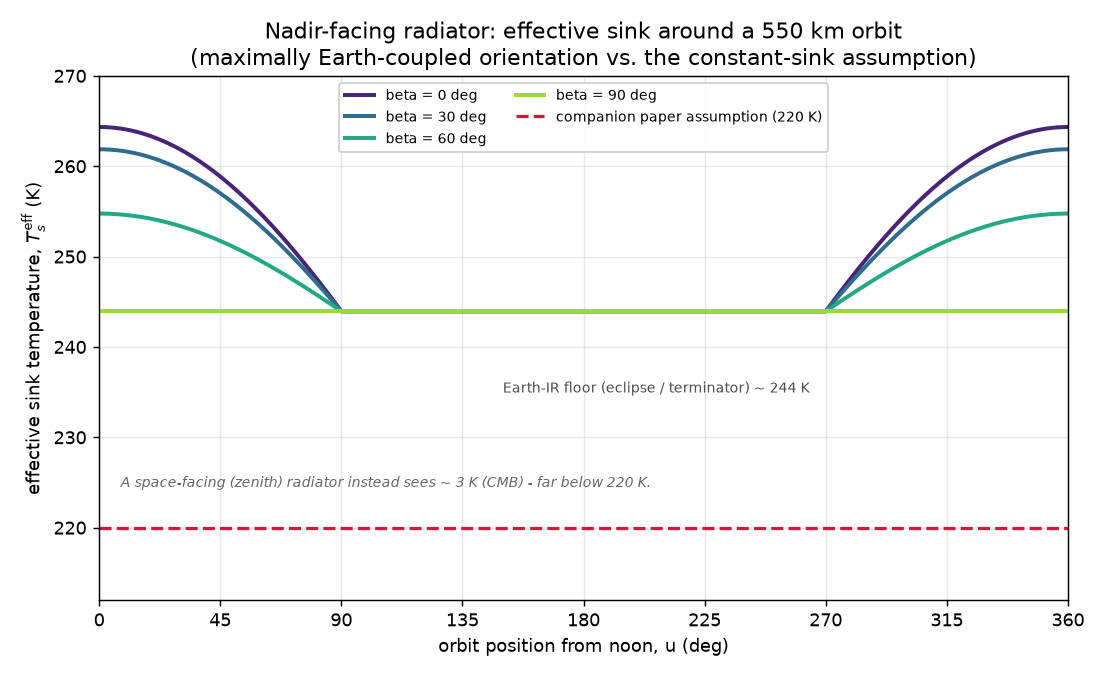
\includegraphics[width=0.82\linewidth]{results/figures/effective_sink_vs_orbit.png}
\caption{Illustrative effective-sink temperature $\Ts$ around a $550$~km orbit for
a \emph{nadir-facing} radiator at several orbit beta angles. For this fixed
nadir attitude the Earth view factor is constant over the orbit; the phase
variation shown is driven by the subpoint-albedo term (Section~\ref{sec:sink}),
and vanishes toward $\beta=90^{\circ}$. The figure illustrates that the radiated-against
environment breathes with orbital position; the orientation-dependent view-factor
effect that drives the correction of Section~\ref{sec:correction} is a separate,
larger effect for a sun-tracking panel.}
\label{fig:sink}
\end{figure}

\subsection{Exact tilted-plate-to-sphere view factor}

Treat Earth as a uniform Lambertian sphere subtending angular radius
$\theta = \arcsin(R_{\oplus}/r)$ at orbital radius $r$, centered on nadir, and let
$\gamma$ be the angle between the plate normal and nadir. For a differential planar
element---an effectively exact approximation for a spacecraft panel, whose
dimensions are negligible relative to $r$---the configuration factor is the
cosine-weighted solid angle over the part of the disk above the plate's
horizon~\cite{howell}. It has the closed limiting forms
\begin{equation}
F(\gamma) =
\begin{cases}
\cos\gamma\,\sin^{2}\theta, & \gamma \le \tfrac{\pi}{2}-\theta \quad(\text{Earth fully above the horizon}),\\[4pt]
0, & \gamma \ge \tfrac{\pi}{2}+\theta \quad(\text{Earth fully set}),
\end{cases}
\label{eq:vf}
\end{equation}
and for the intermediate regime $\tfrac{\pi}{2}-\theta<\gamma<\tfrac{\pi}{2}+\theta$
the horizon clips the disk. The edge-on case $\gamma=\tfrac{\pi}{2}$---the paper's
headline geometry---admits the closed form
\begin{equation}
F\!\left(\tfrac{\pi}{2}\right) = \frac{\theta-\sin\theta\cos\theta}{\pi},
\label{eq:edge}
\end{equation}
obtained by integrating the cosine-weighted solid angle over the half of the disk
above the horizon. At $550$~km, $\theta=\arcsin(6371/6921)$ and
\eqref{eq:edge} gives $F(\tfrac{\pi}{2})=0.257773$ per face. The package computes
the general intermediate regime by a fixed $48$-node piecewise Gauss--Legendre
rule, split at the horizon crossings, with a demonstrated absolute error of order
$10^{-9}$ against independent checks; at edge-on it reproduces~\eqref{eq:edge} to
$<\!10^{-6}$, so the headline value is
independently checkable from~\eqref{eq:edge} without the software.

McCalip's model instead approximates $F$ by a cosine-of-tilt expression with a
lower floor at $5\%$ of the nadir value: per face,
$F_{\mathrm{heur}}(\gamma)=F_{\mathrm{nadir}}\cos\gamma$ for $\cos\gamma>0$ and
$F_{\mathrm{nadir}}\cdot0.05$ otherwise, with
$F_{\mathrm{nadir}}=\sin^{2}\theta$. Near nadir this agrees with~\eqref{eq:vf} to
leading order. Near the horizon the true factor approaches a small but nonzero
grazing value while the heuristic collapses onto its arbitrary floor.

\section{Replication and the edge-on correction}\label{sec:correction}

\subsection{Faithful replication}

An independent Python port of McCalip's \texttt{static/js/math.js}---using his exact
constants, including his truncated $\sig=5.67\times10^{-8}$ and rounded deep-space
temperature $T_{\mathrm{space}}=3$~K---matches a frozen Node regeneration of his
original code (pinned commit \texttt{d1e4238}) to a maximum relative error of
$\sim\!4\times10^{-14}$ across all $297$ compared values in eleven parameter cases:
floating-point roundoff. The model is replicated, not approximated, and the
replication target is pinned so it cannot drift.

\subsection{The default geometry is edge-on}

McCalip's default is a sun-tracking bifacial panel at $\beta=90^{\circ}$ and
$550$~km. At $\beta=90^{\circ}$ the Sun is normal to the orbit plane; a
sun-tracking panel therefore holds its face normal out of the orbit plane, while
nadir lies in the plane, so the panel normal is $90^{\circ}$ from nadir
(Figure~\ref{fig:geom}). Each face sees Earth edge-on for the entire orbit---the
worst case for the cosine-of-tilt heuristic, and the default.

\begin{figure}[t]
\centering
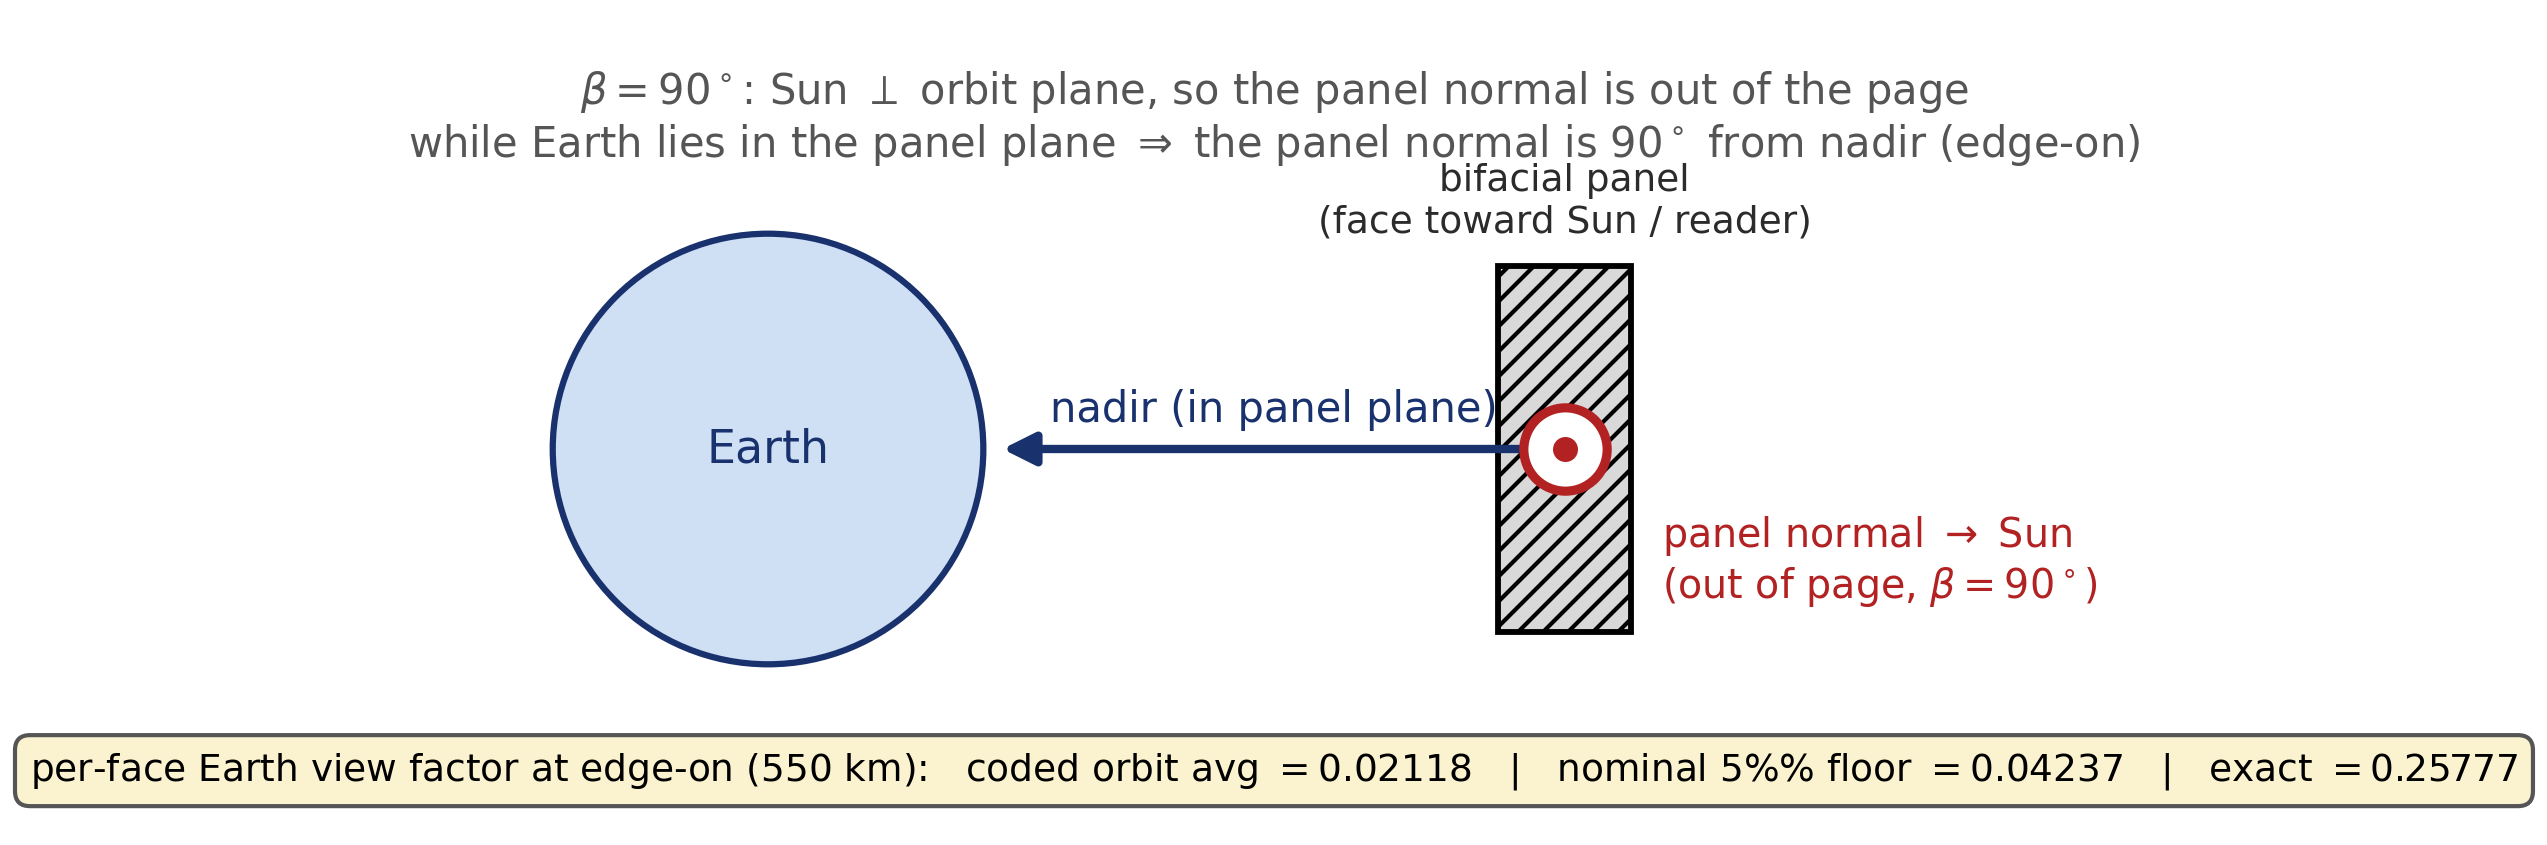
\includegraphics[width=0.86\linewidth]{results/figures/edge_on_geometry.png}
\caption{Why the default geometry is edge-on. At $\beta=90^{\circ}$ the Sun is
perpendicular to the orbit plane, so a sun-tracking panel's normal points out of
the plane while Earth (nadir) lies within it---the panel normal is $90^{\circ}$
from nadir. The three per-face Earth view factors in the callout are computed from
the version-pinned package: the actual coded orbit average ($0.02118$), the
nominal $5\%$ floor ($0.04237$), and the exact edge-on value ($0.25777$).}
\label{fig:geom}
\end{figure}

Three per-face view factors must be distinguished at the edge-on default
(Table~\ref{tab:vf}). The model's \emph{intended} floor is $5\%$ of nadir,
$0.05\times0.84738=0.04237$. Its \emph{actual} orbit-averaged output is $0.02118$:
at $\beta=90^{\circ}$ the code evaluates $\cos(90^{\circ})$ as $\approx6.12\times
10^{-17}$ rather than exact zero, so in the $72$-point orbit loop roughly half the
samples take the tiny-positive-cosine branch and return a value near zero while the
other half take the nonpositive branch and return the floor; the average is almost
exactly half the floor. The \emph{exact} edge-on value is $0.25777$. Thus the exact
factor exceeds the coded output by $12.2\times$ and the intended floor by
$6.1\times$.

\begin{table}[t]
\centering
\caption{Per-face Earth view factor at the edge-on default ($\beta=90^{\circ}$,
$550$~km), and the equilibrium-temperature obtained by feeding each value (both
faces) through McCalip's own heat balance, changing nothing else.}
\label{tab:vf}
\begin{tabular}{lrr}
\toprule
Per-face Earth view factor & value & heat-balance $T_{\mathrm{eq}}$ (K) \\
\midrule
Actual coded $\beta=90^{\circ}$ orbit average & $0.02118447$ & $335.749538$ \\
Nominal intended $5\%$ floor                   & $0.04236893$ & $336.332909$ \\
Exact edge-on view factor~\eqref{eq:edge}      & $0.25777283$ & $342.099222$ \\
\bottomrule
\end{tabular}
\end{table}

\subsection{The correction and its decomposition}

Substituting the exact per-face view factor into McCalip's own heat balance, and
changing nothing else, moves his default coded equilibrium temperature
\begin{equation}
\begin{aligned}
335.749538\ \mathrm{K}\ (\text{coded, replicated})
&\ \longrightarrow\ 342.099222\ \mathrm{K}\ (\text{exact edge-on VF}),\\[2pt]
\Delta T &= +6.349684\ \mathrm{K}.
\end{aligned}
\label{eq:headline}
\end{equation}
This is the correction to the public code \emph{as executed}. It decomposes
cleanly (Table~\ref{tab:decomp}): replacing the intended $5\%$ floor by the exact
geometry accounts for $+5.766313$~K (a model-form geometric error), and the
remaining $+0.583371$~K is the floating-point branch artifact in the orbit average
described above (a numerical implementation effect, not a geometric-model error). A
self-consistency check confirms the attribution: feeding McCalip's own view
factors back through the same heat-balance code reproduces his number to roundoff,
so the shift is due to the view factor and not to any incidental difference in the
balance.

\begin{table}[t]
\centering
\caption{Decomposition of the headline correction at the edge-on default. The
$+6.35$~K is the correction to the actual coded output; it separates into a
model-form geometric correction (intended floor $\to$ exact) and an
implementation edge-case artifact.}
\label{tab:decomp}
\begin{tabular}{lr}
\toprule
Comparison & $\Delta T$ (K) \\
\midrule
Actual coded output $\to$ exact geometry          & $+6.349684$ \\
\quad of which: nominal $5\%$ floor $\to$ exact (model-form geometry) & $+5.766313$ \\
\quad of which: branch artifact (coded $\to$ nominal floor)            & $+0.583371$ \\
\bottomrule
\end{tabular}
\end{table}

The correction is positive at every sampled orbit beta angle, because a sun-tracking
panel's faces, averaged over the orbit, couple to Earth more strongly than the
heuristic reports; across the evaluated range $\beta\in[0^{\circ},90^{\circ}]$ the
exact orbit-averaged bifacial Earth coupling exceeds the heuristic result, so the
temperature correction stays positive at every sampled $\beta$, and increases
monotonically on a dense grid (step $0.5^{\circ}$ over $[0^{\circ},90^{\circ}]$;
minimum sampled increment $+1.06\times10^{-4}$~K), beyond the displayed grid of
Table~\ref{tab:beta} and Figure~\ref{fig:beta}. We claim monotonicity at the
sampled points; continuous monotonicity between samples is not separately proved.

\begin{table}[t]
\centering
\caption{Equilibrium-temperature correction versus orbit beta angle, from
substituting the exact per-face Earth view factor into McCalip's own heat balance
(i.e. relative to his coded output at each $\beta$). The six-decimal values
elsewhere in this paper are computational fingerprints for reproducibility, not
claims of physical accuracy.}
\label{tab:beta}
\begin{tabular}{rrrr}
\toprule
$\beta$ (deg) & coded $T_{\mathrm{eq}}$ (K) & exact-VF $T_{\mathrm{eq}}$ (K) & correction (K) \\
\midrule
0  & 349.58 & 351.53 & $+1.94$ \\
15 & 348.94 & 350.98 & $+2.04$ \\
30 & 347.12 & 349.53 & $+2.41$ \\
45 & 344.42 & 347.63 & $+3.22$ \\
60 & 341.28 & 345.66 & $+4.38$ \\
75 & 338.24 & 343.79 & $+5.55$ \\
90 & 335.75 & 342.10 & $+6.35$ \\
\bottomrule
\end{tabular}
\end{table}

\begin{figure}[t]
\centering
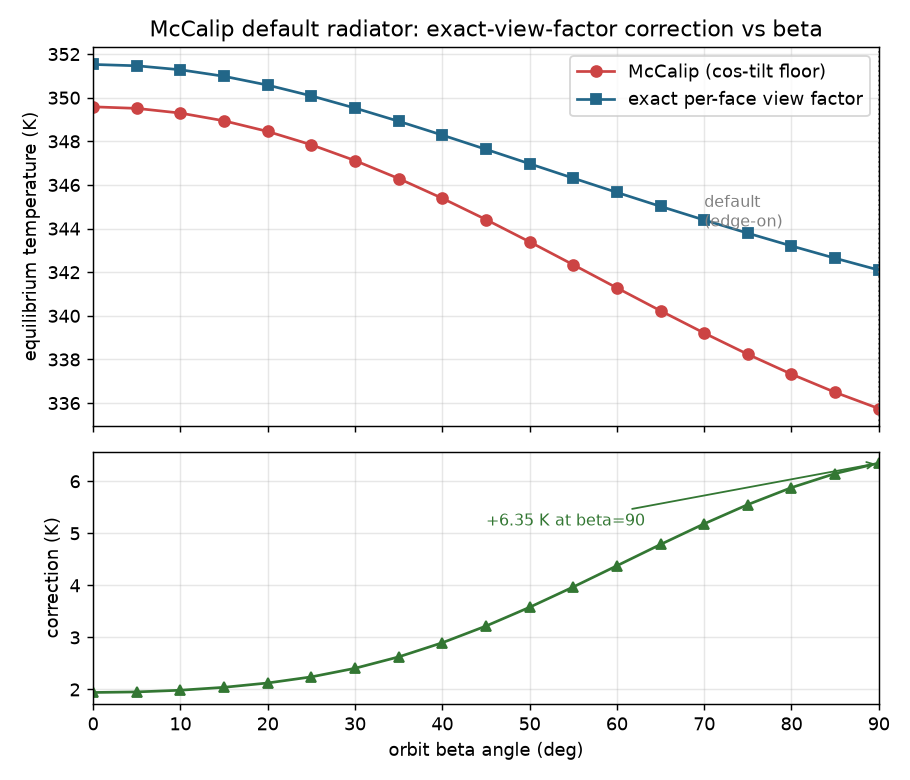
\includegraphics[width=0.78\linewidth]{results/figures/mccalip_beta_correction.png}
\caption{On the evaluated $0.5^{\circ}$ beta grid, the equilibrium-temperature
correction grows monotonically toward the edge-on default. As $\beta$ increases, the sun-tracking panel spends the orbit
closer to the edge-on regime, where the heuristic's orbit-averaged error is
largest---so the implied temperature error is largest exactly where the model is
operated.}
\label{fig:beta}
\end{figure}

\begin{remark}
The sign is intuitive. Underestimating the Earth view factor underestimates
absorbed Earth IR and albedo, understating the environmental load and hence the
temperature the panel must reach to reject it; correcting the view factor upward
raises the predicted temperature.
\end{remark}

\section{Orbit-coupled effective sink}\label{sec:sink}

The static correction fixes one point; a flight panel sweeps a range. We model the
effective sink around the orbit as $\Ts(u)$, with orbital phase
$u\in[0^{\circ},360^{\circ})$, combining the phase-independent Earth-IR term and a
reflected-solar (albedo) term driven by a subpoint-albedo factor
$\max(0,\cos\beta\cos u)$, both weighted by the exact view factor of
Section~\ref{sec:vf}; environmental flux conventions follow standard
references~\cite{spenvis}. The orbit mean of the albedo factor has the closed form
$\langle\max(0,\cos\beta\cos u)\rangle = \cos\beta/\pi$ for
$\beta\in[0^{\circ},90^{\circ}]$, a grid-free reference for the environmental drive
used in the convergence checks of Section~\ref{sec:transient}.

We flag one model-form limitation explicitly. The reflected-solar term is a
\emph{subpoint} approximation: it samples reflectance only at the sub-satellite
point, so it nulls albedo whenever the subpoint is dark and, at $\beta=90^{\circ}$,
reports zero orbit-averaged albedo and a phase-independent sink. A disk-integrated
model accounting for the sunlit Earth crescent within the radiator's field of view
would not vanish there. The subpoint factor is retained as a documented
approximation for the relative, orbit-averaged behavior we report, not asserted as
physics; a disk-integrated replacement is left to future work.

\section{Transient extension and the averaging-load bias}\label{sec:transient}

\subsection{One-node model}

A real radiator panel has thermal mass and cannot follow the orbit-varying sink
instantaneously; it lags and ripples. We model this with a one-node energy balance
per unit area,
\begin{equation}
C\,\frac{dT}{dt} = q_{\mathrm{load}} - \eps\sig\big(T^{4}-\Ts(t)^{4}\big),
\label{eq:onenode}
\end{equation}
with $C$ the areal heat capacity (J\,m$^{-2}$\,K$^{-1}$) and $q_{\mathrm{load}}$
the internal waste-heat flux. Equation~\eqref{eq:onenode} is integrated with
fixed-step RK4 and marched to a periodic steady state.
Figure~\ref{fig:transient} shows the converged temperature history.

\begin{figure}[t]
\centering
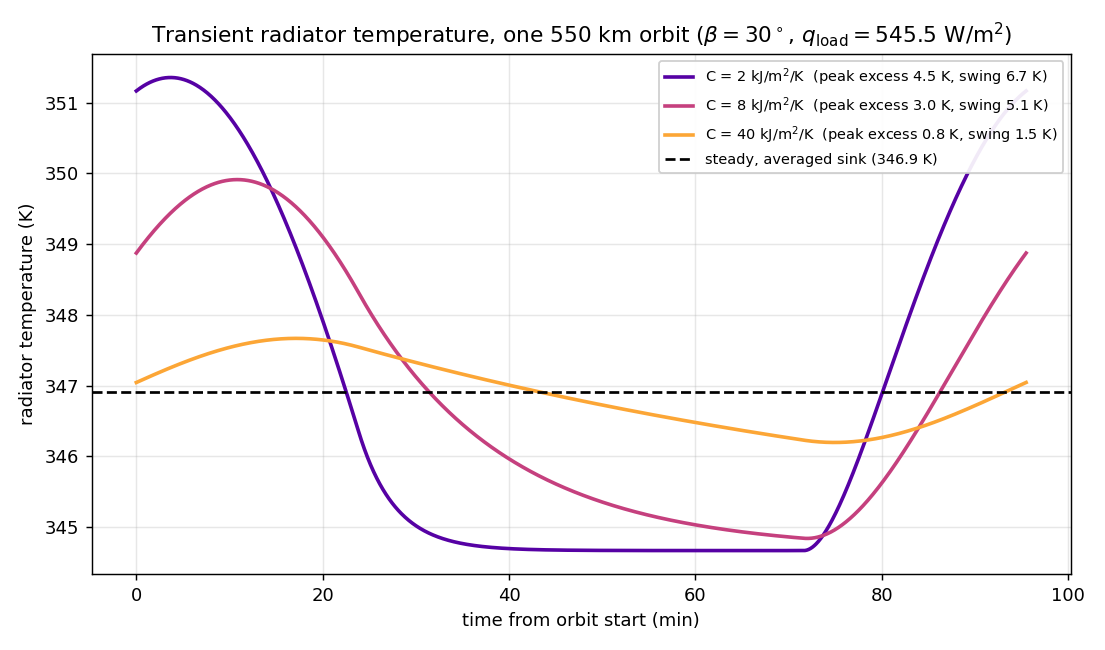
\includegraphics[width=0.82\linewidth]{results/figures/transient_temperature_b30.png}
\caption{One-node panel temperature over a converged orbit at periodic steady
state ($550$~km, $\beta=30^{\circ}$, $q_{\mathrm{load}}=545.5$~W\,m$^{-2}$, the
same point as Table~\ref{tab:bias}), for three areal heat capacities. Thermal mass
turns the sink swing into a damped, phase-lagged ripple; the peak excess over the
steady-state sizing temperature, not the mean, is the operationally relevant
quantity.}
\label{fig:transient}
\end{figure}

\subsection{The averaging-load bias}

Does sizing a radiator at the orbit-averaged sink mis-estimate its behavior? At
periodic steady state, integrating~\eqref{eq:onenode} over one orbit makes the
stored-energy change vanish, so energy balance forces the fourth-power mean to
equal the steady value exactly,
\begin{equation}
\langle T^{4}\rangle = \frac{q_{\mathrm{load}}}{\eps\sig} + \langle (\Ts)^{4}\rangle
= T_{\mathrm{steady}}^{4},
\label{eq:jensen}
\end{equation}
with $T_{\mathrm{steady}}$ the steady solution at the fourth-power-averaged sink.
Because $x^{1/4}$ is concave, the power-mean inequality gives
$\langle T\rangle \le \langle T^{4}\rangle^{1/4} = T_{\mathrm{steady}}$: the
arithmetic-mean temperature sits at or below the steady value. The steady,
averaged-load sizing therefore does not under-predict the mean. What it misses is
the \emph{peak}: any nonzero periodic ripple necessarily carries the panel above
$T_{\mathrm{steady}}$ for part of each orbit (if the waveform is constant---as the
subpoint model becomes at $\beta=90^{\circ}$---the peak, mean, and steady values
coincide and there is no excess). The peak excess is the engineering-relevant
penalty.

Table~\ref{tab:bias} reports both quantities at a representative operating point
across a range of areal heat capacity. The signed mean bias is small and
nonpositive, as~\eqref{eq:jensen} requires; the peak excess is positive and grows
as thermal mass falls, from $0.8$~K for a heavy panel to $4.5$~K for a light one.
The identity~\eqref{eq:jensen} is verified numerically to the solver tolerance at
every case.

\begin{table}[t]
\centering
\caption{Averaging-load bias at $550$~km, $\beta=30^{\circ}$,
$q_{\mathrm{load}}=545.5$~W\,m$^{-2}$. ``Mean bias'' is
$\langle T\rangle - T_{\mathrm{steady}}$ (nonpositive, per~\eqref{eq:jensen});
``peak excess'' is $T_{\max}-T_{\mathrm{steady}}$. $\tau/P$ is the radiative time
constant over the orbital period.}
\label{tab:bias}
\begin{tabular}{rrrrr}
\toprule
$C$ (J\,m$^{-2}$K$^{-1}$) & mean bias (K) & peak excess (K) & swing (K) & $\tau/P$ \\
\midrule
2000  & $-0.028$ & $4.45$ & $6.69$ & $0.04$ \\
8000  & $-0.014$ & $3.01$ & $5.07$ & $0.16$ \\
40000 & $-0.001$ & $0.77$ & $1.47$ & $0.81$ \\
\bottomrule
\end{tabular}
\end{table}

\subsection{Convergence certificate}

Because the periodic steady state and its peak are the load-bearing quantities,
the solver returns a result only when it is certified along three independent
axes: periodic closure (start-to-end orbit temperature change below tolerance); a
scale-aware energy balance (the orbit-mean net flux, as an equivalent temperature
error, below tolerance, which catches a high-thermal-inertia trap that closure
alone misses); and temporal resolution (independently converged solutions at $N$,
$2N$, and $4N$ steps per orbit are compared by a grid-free analytic
forcing-quadrature check, a direct $N\!\to\!4N$ comparison, and a pointwise
waveform comparison on a common phase grid, with a conservative safety margin). The
temporal residual is reported as a refinement-based error estimate rather than a
guaranteed bound, and peak-phase drift is reported separately because an amplitude
bound does not bound the time of the peak. These checks are what let the numbers in
Table~\ref{tab:bias} be quoted without hidden under-resolution.

\section{Verification, reproducibility, and scope}\label{sec:scope}

The claims here occupy specific, deliberately limited levels of a
verification-and-validation hierarchy~\cite{oberkampf}. \emph{Mathematical}
verification (the equations follow from the assumptions) and \emph{software}
verification (the code computes them) are covered by the package's assertion suite
and by the paper-specific verification script of Section~\ref{sec:availability}.
\emph{Cross-model} verification (independent implementations of the \emph{same}
model agree) is covered two ways: our replication of McCalip's model against his
SHA-256-pinned, semantically regenerated original, and our exact view factor
checked both against an independent integrator and against the closed
form~\eqref{eq:edge}. The headline result of Section~\ref{sec:correction} is a
cross-model verification statement: our exact geometry corrects his coded geometry
within his own balance.

We do \emph{not} claim \emph{model-form} validation (assumptions match physical
benchmarks) or \emph{system} validation (predictions match hardware or flight
data). The subpoint-albedo approximation and the sun-shielded attitude assumption
are model-form gaps, held open and labeled; closing them would require the kind of
detailed environmental heat-load and view-factor modeling described in standard
spacecraft thermal-analysis practice~\cite{nasaguidebook}. We identified no publicly available
flight data for this specific orbital-data-center radiator configuration as of June
2026, and we assert no validation against any.

On methodology: the implementation was developed and hardened through an
author-directed adversarial review process in which an AI system (GPT-5.5 with a
computer-algebra plugin) performed independent re-derivation, counterexample
search, and symbolic checks across successive revisions, ending without a
remaining flagged defect. That process is a software-review and reproducibility
record---the review reports are archived as software-review artifacts---and not
external scholarly peer review or evidence of physical validation; the reviewer
was an AI system operating under the author's direction, not an independent
institution or journal referee.

\section{Code and data availability}\label{sec:availability}

The model, tests, frozen oracle, figures, and a paper-specific verification script
are openly available in the project repository
\href{https://github.com/dan-lee-odinson/orbital-thermal-bounds}{\texttt{github.com/dan-lee-odinson/orbital-thermal-bounds}}
at release \texttt{v1.0.0}, immutable commit
\texttt{322fc44db8dc175450ac2e9eb918fe3a1758b2b1} (a Zenodo software DOI will be
minted at archival). The package targets Python $\ge 3.10$ with \texttt{numpy}
(and \texttt{CoolProp==7.2.0} for the optional coolant screen); the McCalip oracle
is regenerated with Node ($\ge 18$). To reproduce:
\begin{verbatim}
    pip install -e ".[fluids]"
    python verify_paper3.py   # decomposition, Tables 1-4, Eq. (5)
    pytest                    # full suite + SHA-256 oracle freeze
\end{verbatim}
\texttt{verify\_paper3.py} is pinned to \texttt{orbital-thermal==1.0.0} and
recomputes the view-factor decomposition (Table~\ref{tab:vf}), the three balances
and decomposition (Table~\ref{tab:decomp}), the beta-correction table
(Table~\ref{tab:beta}), the dense-grid monotonicity increment, and the periodic
identity~\eqref{eq:jensen} with the full Table~\ref{tab:bias} rows; the McCalip
replication against the SHA-256-pinned Node oracle is locked separately by the
package suite (\texttt{tests/test\_mccalip\_replication.py}, oracle pinned at
upstream commit \texttt{d1e4238d3d3f4924e5ca65bafbd4ba5b39af2eb8}, MIT). Each
figure and table is regenerated by a named script: Figure~\ref{fig:sink} by
\texttt{scripts/plot\_effective\_sink.py}, Figure~\ref{fig:geom} by
\texttt{scripts/plot\_edge\_on\_geometry.py}, Figure~\ref{fig:beta} by
\texttt{scripts/plot\_mccalip\_correction.py}, and Figure~\ref{fig:transient}
by \texttt{scripts/plot\_transient.py} (at $\beta=30^{\circ}$).

\section{Conclusion}\label{sec:conclusion}

A prominent public model of orbital data-center radiator behavior is internally
reproducible under its stated assumptions but, at its own default geometry, its
Earth view factor is wrong by a large factor. Replacing the coded value with the
exact tilted-plate-to-sphere view factor, and changing nothing else, raises the
predicted edge-on equilibrium temperature by $6.35$~K, from $335.75$~K to
$342.10$~K. That correction to the code as executed separates into a $+5.77$~K
model-form geometric error---replacing the intended $5\%$ floor by the exact
geometry---and a $+0.58$~K floating-point edge-case artifact in the orbit average;
the correction is positive at every sampled $\beta$ and monotone on the evaluated
$0.5^{\circ}$ grid, and largest at the default.
Extending the static balance to an orbit-coupled transient model shows that a
steady, averaged-load sizing does not under-predict the mean panel
temperature---energy balance pins $\langle T^{4}\rangle=T_{\mathrm{steady}}^{4}$,
so the mean sits at or below steady---but under-predicts the orbital peak by up to
several kelvin for a light panel. Both results are reproducible and machine
verified, and both are offered as cross-model verification, not as validation
against this proposed orbital-data-center radiator configuration, for which we
found no public flight data. For a temperature architecture in which the rejection
temperature enters the required area quartically, a several-kelvin error at the
design point and a multi-kelvin unmodeled peak are not rounding; they are the kind
of margin a flight design has to keep.

\section*{Acknowledgments}

This work was produced through an author-directed, iterative, adversarial workflow
across multiple AI systems: derivation and implementation with Claude (Anthropic),
literature-armed review with Perplexity, and an eight-round software review with
independent computer-algebra verification by GPT-5.5 with the Wolfram plugin,
concluding without a remaining flagged defect. The author directed the work and
takes responsibility for the result. The supporting software, test suite, frozen
oracle, verification script, and figures are openly available in the project
repository; the software-review reports are archived alongside them.

\begin{thebibliography}{9}
\bibitem{paper1} D.~Lee-Odinson, ``Thermodynamic Bounds and Mass-Trade Criteria
for Heat Rejection in Orbital Data Centers,'' Zenodo (2026),
\href{https://doi.org/10.5281/zenodo.20650893}{10.5281/zenodo.20650893}.
\bibitem{paper2} D.~Lee-Odinson, ``The AI1 Design Point: A Bounds-Based Analysis
of SpaceX's Orbital Data-Center Satellite,'' Zenodo (2026),
\href{https://doi.org/10.5281/zenodo.20670772}{10.5281/zenodo.20670772}.
\bibitem{dcd2026} S.~Moss, ``SpaceX details AI1 satellite `data center,' claims
150kW peak compute,'' \emph{Data Center Dynamics}, June~9, 2026,
\url{https://www.datacenterdynamics.com/en/news/spacex-details-ai1-satellite-data-center-claims-150kw-peak-compute/}.
(Announcement-week coverage carrying the quoted Musk and Dahl statements; secondary
source.)
\bibitem{toms2026} L.~James, ``Elon Musk's first-gen orbital data center
craft\ldots AI1 satellite compute payload is 120 kW, peaks at 150 kW,''
\emph{Tom's Hardware}, June~9, 2026,
\url{https://www.tomshardware.com/tech-industry/spacex-details-its-ai1-compute-satellite}.
(Secondary source.)
\bibitem{mccalip} A.~McCalip, ``Space Datacenters'' thermal/cost model, source file
\texttt{static/js/math.js}, repository \texttt{andrewmccalip/thoughts}, pinned
commit \texttt{d1e4238d3d3f4924e5ca65bafbd4ba5b39af2eb8} (MIT license; accessed
June 2026).
\bibitem{howell} J.~R. Howell, M.~P. Mengüç, K.~Daun, and R.~Siegel,
\emph{Thermal Radiation Heat Transfer}, 7th ed. (CRC Press, 2020); see also
Howell's catalog of radiation configuration factors.
\bibitem{oberkampf} W.~L. Oberkampf and C.~J. Roy, \emph{Verification and
Validation in Scientific Computing} (Cambridge University Press, 2010).
\bibitem{nasaguidebook} NASA, \emph{Passive Thermal Control Engineering
Guidebook}, v4.0, NTRS 20230013900 (2023).
\bibitem{spenvis} ESA, ``Satellite irradiation: solar, albedo and Earth infrared
environments,'' SPENVIS background documentation.
\end{thebibliography}

\end{document}
